\documentclass[a4paper,12pt]{article}

\usepackage[english]{babel}
\usepackage[T1]{fontenc}
\usepackage[utf8]{inputenc}
\usepackage{amsmath}
\usepackage{amsthm}
\usepackage{graphicx}

\usepackage{geometry}
\geometry{total={210mm,297mm},
left=20mm, right=20mm,
bindingoffset=0mm,
top=20mm, bottom=20mm}

\usepackage[
  pdftitle={Homework 5},
  pdfauthor={William Jagels},
  colorlinks=true,linkcolor=blue,urlcolor=blue,citecolor=blue,bookmarks=true,
bookmarksopenlevel=2]{hyperref}

\usepackage{titlesec}
\titlelabel{\thetitle.\quad}

\def\code#1{\texttt{#1}}

\title{Homework 5}

\author{William Jagels}

\date{\today}

\begin{document}
\maketitle

\section{Exercise 1.10a}
$\{w| w$ contains at least three 1s$\}*$

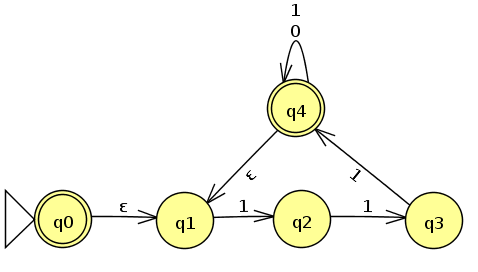
\includegraphics[width=15cm]{q1}

\section{Exercise 1.10b}
$\{w| w$ contains at least two $0$s and at most one $1\}*$

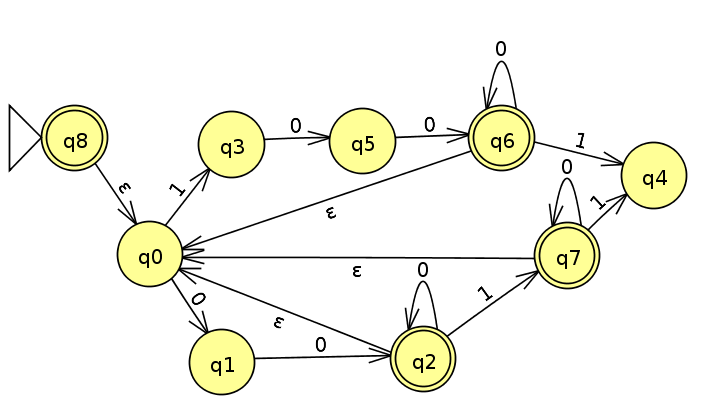
\includegraphics[width=15cm]{q2}

\section{Exercise 1.29b}
$A_2 = \{www| w \in \{a, b\}^*\}$

Assume $A_2$ is regular.
Let $s=a^pba^pba^pb$ and divide into 3 pieces, $s=xyz, |xy| \leq p$.
Therefore, xy only contains symbol a.
As $|y|>0$, set $y=a^k$, $k>0$.
$xy^2z = a^{p+k}ba^pba^pb$ results in a string not in $A_2$.
This is a contradiction, and cannot be pumped.

\section{Exercise 1.46a}
$\{0^n 1^m 0^n | m, n \geq 0\}$

We can apply the pumping lemma with $s=0^p10^p$ and $s=xyz$.
$xy$ contains only zeroes.
Assign $y=0^k$ and $k \geq 0$.
Now, $xy^0z = 0^{p-k}10^p$ cannot be in the language.
Because of this, the language cannot be regular.

\section{Exercise 1.46c}
$\{w| w \in \{0,1\} *$ is not a palindrome$\}$

In order to determine whether or not a string is a palindrome, we need to have memory.
Reversing the string and comparing it to the original is impossible given that a finite
automata has no memory.
This would require infinitely many states, therefore the language is not regular.

\section{Exercise 1.46d}
$\{wtw| w, t \in \{0,1\}^+ \}$

We can apply the pumping lemma with $s=0^p10^p$ and $s=xyz$.
$xy$ contains only zeroes.
Assign $y=0^k$ and $k > 0$ due to the $+$ operator.
Now, $xy^0z = 0^{p-k}10^p$ cannot be in the language.
Because of this, the language cannot be regular.

\section{Exercise 1.47}
Let $\Sigma = \{1, \#\}$ and let

$Y = \{w| w = x 1 \#x 2 \# \cdots \#x_k$ for $k \geq 0,$ each $x_i \in 1^* ,$ and $x_i \neq x_j$ for $i \neq j\}$

Prove that $Y$ is not regular.

The language $Y$ requires that there be a memory of encountered strings between delimiters.
There would need to be infinitely many states to accomplish this, therefore this is
not a regular language as a DFA is unable to recognize it.

\section{Exercise 1.49}
\subsection{Part A}
Let $B = \{1^k y| y \in \{0, 1\}^*$ and $y$ contains at least $k$ $1$s, for $k \geq 1\}$.
Show that $B$ is a regular language.

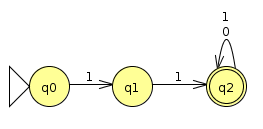
\includegraphics[width=6cm]{q8}

With the above NFA, we can recognize any number of $1$s more than zero.
Therefore, the language is regular.
To require a different number of $1$s, just add more states between $q0$ and $q2$.

\subsection{Part B}
Let $C = \{1^k y| y \in \{0, 1\}^*$ and $y$ contains at most $k$ $1$s, for $k \geq 1\}$.
Show that $C$ isn't a regular language.

$C$ is not a regular language because it would violate the pumping lemma.
$s = 1^p0^p1^p \in C$, $s=xyz$, $|xy|\leq p$, $y=1^i$, $i \geq 1$.
Therefore, $xz=1^{p-i}0^p1^p\in C$ which contradicts.

\section{Show that $\{0^n1^m2^k | k$ divides $n + m\}$ is not regular}
As there are infinitely many natural numbers, there are infinitely many $k$s, $n$s, and $m$s there could be.
This language is infinite and therefore not regular.

\section{Convert the following NFA to a DFA}
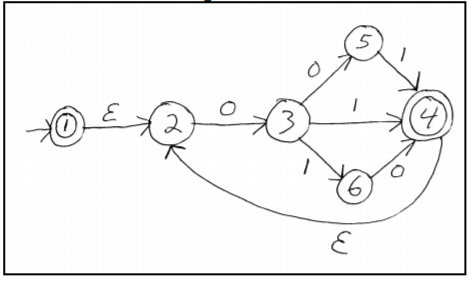
\includegraphics[width=7cm]{q10q}

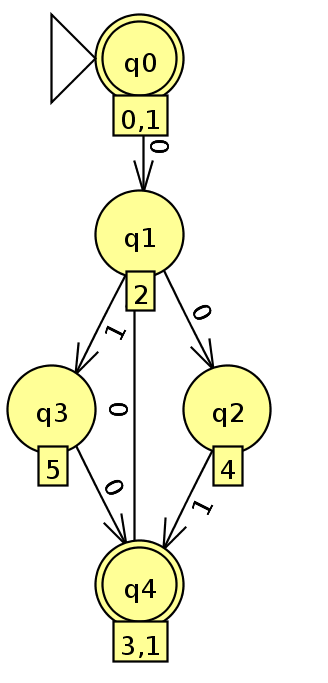
\includegraphics[width=6cm]{q10}

\end{document}
